\documentclass[conference]{IEEEtran}
\IEEEoverridecommandlockouts
% The preceding line is only needed to identify funding in the first footnote. If that is unneeded, please comment it out.
\usepackage{cite}
\usepackage{amsmath,amssymb,amsfonts}
\usepackage{algorithmic}
\usepackage{graphicx}
\usepackage{hyperref}
\usepackage{textcomp}
\usepackage{xcolor}
\def\BibTeX{{\rm B\kern-.05em{\sc i\kern-.025em b}\kern-.08em
    T\kern-.1667em\lower.7ex\hbox{E}\kern-.125emX}}

\makeatletter
\newcommand{\linebreakand}{%
  \end{@IEEEauthorhalign}
  \hfill\mbox{}\par
  \mbox{}\hfill\begin{@IEEEauthorhalign}
}
\makeatother

\begin{document}

\title{Ascribing Machine Learning Classifiers to diagnose the attacks of \textit{Alternaria solani} on Leaves of \textit{Solanum tuberosum}\\}

\author{\IEEEauthorblockN{1\textsuperscript{st} Anurag Dutta}
\IEEEauthorblockA{\textit{Department of Computer Science and Engineering} \\
\textit{Government College of Engineering \& Textile Technology}\\
Serampore, Calcutta, India \\
anuragdutta.research@gmail.com}
\and 
\IEEEauthorblockN{2\textsuperscript{nd} Pijush Kanti Kumar}
\IEEEauthorblockA{\textit{Department of Information Technology} \\
\textit{Government College of Engineering \& Textile Technology}\\
Serampore, Calcutta, India \\
pijush752000@yahoo.com}
\linebreakand 
\IEEEauthorblockN{3\textsuperscript{rd} Ankita De}
\IEEEauthorblockA{\textit{Department of Computer Science and Engineering} \\
\textit{Government College of Engineering \& Textile Technology}\\
Serampore, Calcutta, India \\
ankitade2001@gmail.com}
\and
\IEEEauthorblockN{4\textsuperscript{th} Padmanavan Kumar}
\IEEEauthorblockA{\textit{Department of Computer Science and Engineering}\\
\textit{Kalinga Institute of Industrial Technology}\\
Bhubaneswar, Odisha, India\\
padmanavan2021@gmail.com}
\linebreakand 
\IEEEauthorblockN{5\textsuperscript{th} Shubhangi Dwivedi}
\IEEEauthorblockA{\textit{School of Mathematical and Statistical Sciences}\\
\textit{Indian Institute of Techology, Mandi}\\
Mandi, Himachal Pradesh, India\\
shubhangi.dwivedi176@gmail.com}
\and
\IEEEauthorblockN{6\textsuperscript{th} Krishan Kumar Yadav}
\IEEEauthorblockA{\textit{Department of Mathematics}\\
\textit{SRM Institute of Science and Technology}\\
Ghaziabad, Uttar Pradesh, India\\
Krishankumaryadav222@gmail.com}
}

\maketitle

\begin{abstract}
Following the recent advances in technology, came advanced computational domains like, Internet of Things, Machine Learning, Artificial Intelligence, Data Science, and many more. These fields really tend to help mankind a lot. In this work, we would make use of Machine Learning aspects to perform prediction of diseases in plant. Specifically, spot the Early Blight Disease in the Potato Leaves. The potato plant, \textit{Solanum tuberosum}, is a significant crop that is grown all over the world and generates large quantities of tubers that are a good source of nutrients. The potato has many medicinal benefits in addition to being a common staple diet. When the fluid out from tubers is consumed in moderation, it can treat gastric ulcers and relieve inflammation and acidity. Two harmful potato diseases, late blight and early blight, are pervasive. Everywhere potatoes are cultivated, both are present. The labels "Early" and "Late" allude to the relative timing of their field emergence, however both disorders might manifest simultaneously. In this work, we would focus on Early Blight. The fungus \textit{Alternaria solani}, that can infect potatoes, tomatoes, several species of the potato genus, and some mustards, is the cause of early blight of potatoes. Young, actively growing plants are rarely impacted by this disease, commonly known as target spot. It first appears on elder leaves. Warm temperatures and heavy humidity foster Early Blight. This disease affects the tuber symptomized by dark, rounded to irregular dots being developed on the tuber. As the disease develops, the flesh of the potatoes commonly becomes water-soaked yellow to greenish yellow. For this work, we have collected a set of nearly 1000 samples of Early Blight affected Potato Leaves. Using that, we have modelled a Machine Learning Classification Paradigm that could potentially predict the occurrence of Early Blight Disease making using of classical classifier algorithms. Medical Science have advanced to a great height. If we could potentially predict the disease, in the early stages, Plant Pathology could stop the menace from occurrence. \\
\end{abstract}

\begin{IEEEkeywords}
Machine Learning, Plant Pathology, \textit{Solanum tuberosum}, \textit{Alternaria solani}
\end{IEEEkeywords}
\section{Introduction}
The potato plant, \textit{Solanum tuberosum} [1], is a significant crop that is grown all over the world and generates large quantities of tubers that are a good source of nutrients. A perennial herbaceous \textit{Solanum tuberosum} [2] can reach a height of about 60 cm. The potato is planted and harvested annually in contemporary farming as an annual species. Plants have tall, pinnate leaves and produce white, pink, blue, or purple blooms with clusters of yellow stamens. Although self-fertilization also occurs, bumblebees and other insects such as them are the primary pollinators of potatoes. Green cherry tomatoes, with or without seeds, are similar to the fruit of \textit{Solanum tuberosum} [3]. Fruits should not be consumed by humans because they are highly harmful because of the \textit{Solanine} [4] alkaloid they contain. The edible part of the potato plant, termed as the tubers, are produced as the plant grows and are bigger underground stems. The only component of this plant that is crucial for commerce is the tuber. In addition to being used in vegetative plant multiplication, tubers retain and preserve nourishment that helps the plant withstand the cold. Ingestion of young potatoes especially potato sprouts can result in a number of symptoms, some of which may be serious. The potato has many medicinal benefits in addition to being a common staple diet. When the liquid out from tubers is consumed in moderation, it can treat gastric ulcers and reduce pain and acidity. However, drinking more potato juice beyond one big potato per day is not recommended because it can be hazardous in high doses. The potato poultice can be applied on haemorrhoids, skin rashes, swellings, and rheumatic joints. Additionally, uncooked potatoes have been used as a cooling plaster for burns and scalds. In India, burns and swollen gums are treated with potato skins being subjected to \textit{ayurveda} [5]. The most common \textit{glycoalkaloids} - toxic substances found in potatoes [6] - are \textit{solanine} and \textit{chaconine} [7]. Other species of the \textit{Solanaceae} plant family [8], such as \textit{Atropa belladonna} [9] \& \textit{Hyoscyamus niger} [10], also possess \textit{Solanine}. Wild potatoes have sufficient amounts of \textit{glycoalkaloid} to have harmful effects on people. Additionally, it was shown that the \textit{glycoalkaloid} content of the tuber increases with age, physical injury, and light exposure, with the largest amounts occurring close beneath the skin. However, because the toxic substances in the plant known are often centered in the green parts of the plants and in the fruits, and because cultivated potato cultivars have lower toxin levels, poisoning from potatoes happens very infrequently. Additionally, it was discovered that the toxin is partially eliminated at high temperatures ($\ge$ 170°C) or while cooking. \\

\textit{Alternaria} [11], also referred to as \textit{Early Blight} [12], is a fungal infection that primarily lives in the soil and harms potato crops. It affects crops all across the world and has long been a problem in Great Britain. Figure 1 shows a referential image of Early Blight Disease in potato. 
\begin{figure}[htbp]
\label{fig1}
\centerline{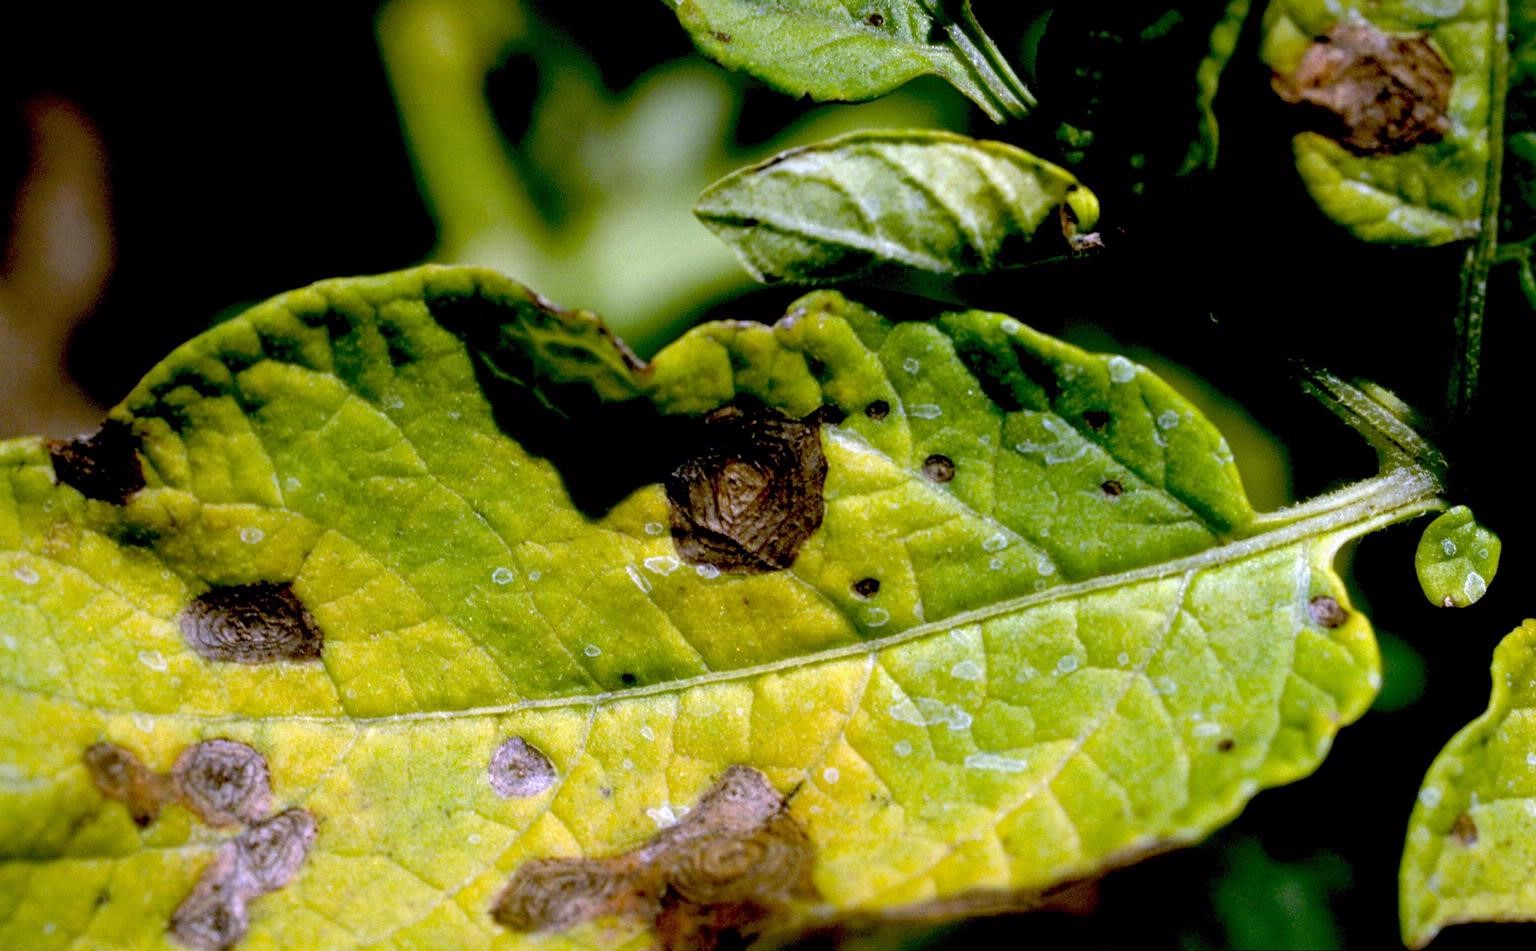
\includegraphics[width = \linewidth]{EarlyBlight}}
\caption{\textit{Early Blight disease in Potato}: Early maturing cultivars are especially vulnerable as the disease first manifests itself on senescent and adult leaf. The principal host plant is the potato, but other solanaceous plants including hairy nightshade and tomatoes can also be severely affected by the disease.}
\end{figure}
If the disease is not treated, it can induce significant leaf loss, which can result in losses in yield of up to 30\%. Warm and rainy conditions favour the illness. The susceptibility of each variety varies. \textit{Alternaria solani} is the main species. \textit{Alternaria alternata} is a different pathogen that harms potatoes and usually infects them later in the growing season. Without a microscope, it is nearly impossible to tell the two species apart. On the leaves, \textit{Alternaria} develops lesions that frequently resemble target spots with concentric rings. These typically though, not always start as tiny black or brown patches on lower leaves, cluster, and then appear a few weeks following emergence. As the disease spreads, this results in the death of the leaf tissue, changing the symptoms over time. Due to the absence of \textit{Alternaria}spores on the leaves, even with a hand lens, and the lack of a distinctive milky ring of sporulation surrounding the lesion on the underside of the leaf, the disease can be distinguished from late blight \textit{Phytophthora infestans} [13]. The diagnosis might be challenging since symptoms can be misinterpreted for \textit{Verticillium wilt} [14] or nutrient deficiencies. Figure 2 shows a potato lead affected by \textit{Verticillium Wilt}. 
\begin{figure}[htbp]
\label{fig2}
\centerline{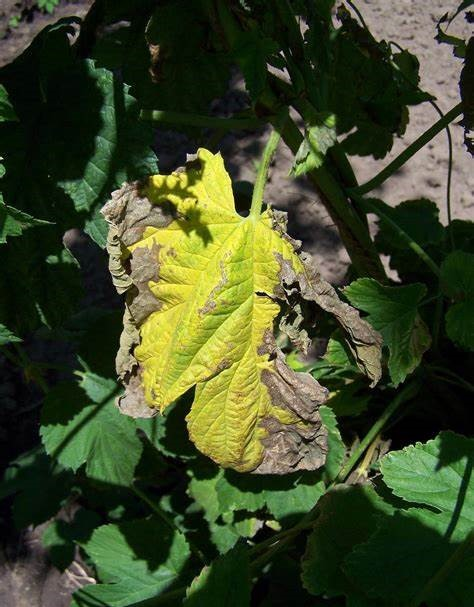
\includegraphics[width = \linewidth]{VerticilliumWilt}}
\caption{\textit{Verticillium Wilt disease in Potato}: One of distinct strains of Verticillium can cause this fungal illness. All U.S. regions that grow potatoes, including Maine, are affected by the disease. Verticillium wilt can reduce tuber size, which can lead to yield losses. Additionally, it may result in stem-end browning and lower tuber quality for the tablestock and chip markets.}
\end{figure}
Particular symptoms are frequently mixed together with manganese toxicity and magnesium insufficiency. Our work, would make use of Machine Learning Model, that would be modelled using a well stacked dataset, with nearly 1000 data points, to predict the potent presence of \textit{Alternaria solani} on Leaves of \textit{Solanum tuberosum}. \\

Although there are few culturally appropriate management strategies, managing field debris will be beneficial. A good weed management strategy, including getting rid of volunteers and other hosts like nightshades, will also lower the amount of \textit{Alternaria}. Extended crop rotations can reduce the occurrence of disease. One can also decrease the effect by not allowing their crop to experience stress. Disease impact is reduced by good crop management, proper fertiliser inputs, and irrigation best practises.
\section{Supervised Learning}
Machine Learning [16] is a branch within Artificial Intelligence (AI) [15] and Computer Science that focuses on using information and algorithms to replicate how humans learn, eventually enhancing the system's accuracy. Machine learning-based products, such as Netflix's recommendation engine and self-driving cars, have become available in recent years as a result of technological advances in storage and processing capacity. Machine learning is an important component of the rapidly increasing study of data science. In data mining projects, algorithms are programmed using mathematical procedures to provide classifications or forecasts and to uncover key insights. Decisions based on these insights, ideally, influence key growth metrics in applications and companies. As big data evolves to emerge and flourish, data scientists will become increasingly in demand. They will be asked to help determine the most important queries and the information required to answer them. Machine Learning Algorithms are typically built using faster solution framework for the development such as TensorFlow and PyTorch. \\ 

UC Berkeley researchers divides the learning mechanism of a ML algorithm into three fundamental components.
\begin{enumerate}
\item A Decision Process
\item An Error Function
\item A Model Optimization Process
\end{enumerate}
The term "supervised learning," [17] which sometimes goes by the name "supervised machine learning," refers to a class of ML that uses existing data instances subjected to model that reliably aims in classifying data and make predictions. The model instantiates its points as input data points are fed into it until it is satisfied to be well fitted. This happens as component of something like the Cross Validator procedure to ensure that the model does not fit too well in training data or too poorly in such. A common example of how supervised learning aids companies is 'Categorizing spam emails'. Neural networks [18], Naïve Bayes, Linear Regression, Logistic Regression, Random Forest, and Support Vector Machines [19] are a few techniques used in supervised learning (SVM). \\

The problem statement that we want to intend is to predict whether a Potato Leaf has got the following disease or not. It's simply a classification based problem, where we will have to train the model in such a way that it can predict the occurrence of the disease, with maximal possible accuracy. Hereby, in our work, the data would be of either of two types,
\begin{enumerate}
\item Affected by Early Blight Disease
\item Health Leaf. 
\end{enumerate}
So, to solve the problem, we will make use of Classical ML Classifiers. 
\section{Classification Algorithms}
Using classification methods, data is classified into classes or categories. It can be carried out using both organised and unstructured data. Multiclass, Multilabel, and Binary Classification are the three types of classification.
\subsection{Logistic Regression}
This type of statistical model, often known as a logit model, is widely used in predictive analytics and categorization. Logistic regression predicts the chance of an event occurring, such as voting or not voting, using a certain dataset of independent factors. Given that the outcome is a likelihood, the range of the dependent variable is 0 to 1. In logistic regression, the possibilities of that happening are translated using the logit formula [20], which is the chance of success divided by the probability of failure. This is also known as the natural logarithm of odds or the log odds. The following formulas represent this logistic function
\begin{equation}
logit(\pi)=\frac{1}{1+e^{-\pi}}
\end{equation}
and
\begin{equation}
ln(\frac{\pi}{1-\pi}) = \beta_0 + \beta_1 \times x_1 + \beta_2 \times x_2 + ... + \beta_k \times x_k
\end{equation}
The dependent or response variable inside this logistic regression equation is $logit(\pi)$, and the independent variable is $x$. This model's beta parameter is usually estimated using maximum likelihood estimation (MLE). This method iteratively tests beta values to get the best log odds fit. Logistic regression maximises the log likelihood function after each iteration to estimate parameters accurately. After obtaining the optimal coefficient(s), the conditional probability of each observation is evaluated, logged, and summarized to give a overhead probability. A probability of less than $\frac{1}{2}$ predicts 0 and more than 0 predicts 1. After computing the model, evaluate its goodness of fit, or ability to predict the dependent variable. The \textit{Hosmer-Lemeshow} test is a well-liked technique for evaluating model fit.
\subsection{Support Vector Machines}
SVM improves accuracy of the model without overfitting its training dataset. SVM works best with thousands of predictor fields. CRM, face and other image identification, genomics, idea retrieval from text mining, surveillance cameras, protein sequence prediction, voice and speech synthesis, and other domains benefit from SVM. SVM uses a high-dimensional feature set to categorise data points that cannot be separated linearly. Data are translated to create a hyperplane representation of a category separator. New data can forecast a record's group. SVM creates a hyper-plane that categorises data. This hyper-plane is a two-dimensional line. SVM plots each dataset item in a $N$-dimensional space. Divide the data using the optimal hyperplane.
\subsection{$k$ Nearest Neighbours}
K-Nearest Neighbour, as a exclusive supervised ML technique, is quite simple. The K-NN algorithm make the assumption that the new case and the old cases are comparable and arranges the new data instance in the category most similar to the existing classes. After storing all data points, the K-NN algorithm categorizes nascent data points by similarity. K-NN can rapidly and reliably classify new data points. Regression can also be done with K-NN, which is usually used for classification. K-NN is non-parametric and makes no data assumptions. This lazy learner algorithm stores the training dataset rather than learning from it immediately. It classifies data using this stored dataset.
\subsection{Random Forest}
The random forest approach generates an uncorrelated forest of decision trees using bagging and feature randomness. Feature randomization, also known as feature bagging or "the random subspace approach," randomises characteristics to reduce decision tree correlation. Random forest techniques require three hyper - parameters before training. These include node size, tree count, and sampled features. Apply the random forest classifier to regression or classification problems. Each decision tree in the random forest ensemble is a bootstrap sample from a training set with replacement. The out-of-bag (oob) sample, which we shall discuss later, is one-third of the training sample. Feature bagging adds randomization, improving dataset diversity and minimising decision tree correlation. Situation dictates prediction. Regression tasks average the decision trees, while classification tasks use the majority vote or most prevalent categorical variable to forecast the class. Cross-validation with the oob sample completes the prediction.
\subsection{Gaussian Naive Bayes}
Naive Bayes, based on the Bayes theorem, is used for many categorization functions. Gaussian naive Bayes is its generalisation. The Gaussian or normal distribution, which just requires the mean and standard deviation for training data, is the easiest to implement. Naive Bayes probabilistic machine learning is useful for categorisation. Document classification, spam filtering, prediction, and more use Naive Bayes. Based on Thomas Bayes' insights, this method is named. The "Nave" technique integrates independent features into its model. Changes to one algorithm feature do not affect other features. The Naive Bayes algorithm is simple and effective. Its probabilistic model makes real-time forecasts with an easily codable algorithm. This algorithm solves real-world problems since it can quickly respond to customer requests. Conditional probability must be understood before studying Nave Bayes and Gaussian Nave Bayes.
\subsection{Decision Tree}
We can describe the choices and the possible outcomes of those selections, covering outputs, input costs, and utilities, using a machine learning approach known as a decision tree. The decision-making algorithm is a member of the supervised learning methods category. It functions with continuous and classified output parameters. In a decision tree, which resembles a flowchart, each leaf node symbolises the individual decision's outcome, while each inner node represents a variable (or feature) of the dataset. The root node is the node that is located at the top of a decision tree diagram. Based on the attribute values that match to the independent qualities, we can segment the data. Recursive partitioning is a technique for breaking up a tree into separate components. The complete structure of this decision tree, which resembles a flowchart, facilitates decision making. It provides a diagrammatic paradigm that perfectly captures how people think and make decisions. Decision trees are simple to study and comprehend due to this flowchart aspect.
\section{Dataset}
The dataset, that we have used in this work is available at \href{https://github.com/Anurag-Dutta/Maneuvering-Machine-Learning-Algorithms-to-presage-the-attacks-of-Alternaria-solani-on-Potato-Leaves/tree/main/dataset}{https://github.com/Anurag-Dutta/Maneuvering-Machine-Learning-Algorithms-to-presage-the-attacks-of-Alternaria-solani-on-Potato-Leaves/tree/main/dataset}. It contains a collection if nearly 1000 images of Potato Leaves affected by Early Blight Disease, and nearly 150 images of Potato Leaves that are healty - being unaffected by any Disease. A few more details about the dataset, drawn from the code are as, 
\begin{verbatim}
import os

path = os.listdir('dataset/')
classes = {'Healthy':0, 'Early Blight':1}

import cv2
X = []
Y = []
for cls in classes:
    pth = 'dataset/'+cls
    for j in os.listdir(pth):
        img = cv2.imread(pth+'/'+j, 0)
        img = cv2.resize(img, (200,200))
        X.append(img)
        Y.append(classes[cls])
        
X = np.array(X)
Y = np.array(Y)

X_updated = X.reshape(len(X), -1)

np.unique(Y)

pd.Series(Y).value_counts()
\end{verbatim}
The output corresponding to the code fragment would be 
\begin{verbatim}
array([0, 1])

1    1000
0     152
dtype: int64
\end{verbatim}
This shows that, the dataset that we are dealing with is composed of a atotal of 1152 data points with either of the labels 0, or 1. \\

The entire code is made available \href{https://github.com/Anurag-Dutta/Maneuvering-Machine-Learning-Algorithms-to-presage-the-attacks-of-Alternaria-solani-on-Potato-Leaves/blob/main/Maneuvering\%20Machine\%20Learning\%20Algorithms\%20to\%20presage\%20the\%20attacks\%20of\%20Alternaria\%20solani\%20on\%20Potato\%20Leaves.ipynb}{here}. 
\section{Results and Conclusion}
In this section, we would conclude our discussions by producing the results. Here, in this work, we made use of numerous ML Algorithms for the Classification of Leaves of \textit{Solanum tuberosum}, being affected by \textit{Alternaria solani} or not. The results are underlying. 
\begin{verbatim}
=======================
[ Logistic Regression ]
=======================

Precision: 0.949238578680203
Recall: 0.9396984924623115
F1 Score: 0.9444444444444445
\end{verbatim}
\begin{verbatim}
==========================
[ Support Vector Machine ]
==========================

Precision: 0.9514563106796117
Recall: 0.9849246231155779
F1 Score: 0.9679012345679012
\end{verbatim}
\begin{verbatim}
==========================
[ k - Nearest Neighbours ]
==========================

Precision: 0.9881656804733728
Recall: 0.8391959798994975
F1 Score: 0.907608695652174
\end{verbatim}
\begin{verbatim}
========================
[ Gaussian Naive Bayes ]
========================

Precision: 0.9788359788359788
Recall: 0.9296482412060302
F1 Score: 0.9536082474226804
\end{verbatim}
\begin{verbatim}
==========================
[ Random Decision Forest ]
==========================

Precision: 0.8873873873873874
Recall: 0.9899497487437185
F1 Score: 0.9358669833729216
\end{verbatim}
\begin{verbatim}
=================
[ Decision Tree ]
=================

Precision: 0.8974358974358975
Recall: 0.8793969849246231
F1 Score: 0.9444444444444445
\end{verbatim}
Here, the maximal F1 Score is contributed by Support Vector Classifier. Figure 3 and 4 shows the Precision Recall Curve, and the Confusion Matrix of the Model, modelled using Support Vector Machine Algorithm. 
\begin{figure}[htbp]
\centerline{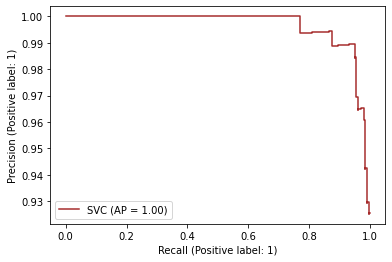
\includegraphics[width = \linewidth]{PRC_SVM}}
\label{fig3}
\caption{Graph showing Precision versus Recall for Support Vector Machine}
\end{figure}
\begin{figure}[htbp]
\centerline{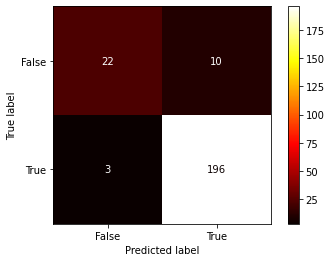
\includegraphics[width = \linewidth]{CM_SVM}}
\label{fig4}
\caption{Confusion Matrix for Support Vector Machine}
\end{figure}
\textbf{\\}

Some scopes of Future Research includes classifying the leaves making use of some better Classifier, or Neural Network, that could potentially give a bump to the performance of the Prediction. 

\begin{thebibliography}{00}
\bibitem{b1} E.-J. Eggers et al., “Neofunctionalisation of the Sli gene leads to self-compatibility and facilitates precision breeding in potato,” \textit{Nature Communications}, vol. 12, no. 1, Jul. 2021, doi: 10.1038/s41467-021-24267-6.
\bibitem{b2} J. A. Foley et al., “Solutions for a cultivated planet,” \textit{Nature}, vol. 478, no. 7369, pp. 337–342, Oct. 2011, doi: 10.1038/nature10452.
\bibitem{b3} L. Ma et al., “A nonS-locus F-box gene breaks self-incompatibility in diploid potatoes,” \textit{Nature Communications}, vol. 12, no. 1, Jul. 2021, doi: 10.1038/s41467-021-24266-7.
\bibitem{b4} J. A. Maga and T. J. Fitzpatrick, “Potato glycoalkaloids,” \textit{C R C Critical Reviews in Food Science and Nutrition}, vol. 12, no. 4, pp. 371–405, Jul. 1980, doi: 10.1080/10408398009527281.
\bibitem{b5} P. A. Maas, “Indian Medicine and Ayurveda,” \textit{The Cambridge History of Science}, pp. 532–550, Dec. 2018, doi: 10.1017/9780511980145.029.
\bibitem{b6} M. Friedman, G. M. McDonald, and M. Filadelfi-Keszi, “Potato Glycoalkaloids: Chemistry, Analysis, Safety, and Plant Physiology,” \textit{Critical Reviews in Plant Sciences}, vol. 16, no. 1, pp. 55–132, Jan. 1997, doi: 10.1080/07352689709701946.
\bibitem{b7} K. TAKAGI, M. TOYODA, Y. FUJIYAMA, and Y. SAITO, “Effect of Cooking on the Contents of $\alpha$-Chaconine and $\alpha$-Solanine in Potatoes,” \textit{Food Hygiene and Safety Science (Shokuhin Eiseigaku Zasshi)}, vol. 31, no. 1, pp. 67-73\_1, 1990, doi: 10.3358/shokueishi.31.67.
‌\bibitem{b8} K. Kubo et al., “Gene duplication and genetic exchange drive the evolution of S-RNase-based self-incompatibility in Petunia,” \textit{Nature Plants}, vol. 1, no. 1, Jan. 2015, doi: 10.1038/nplants.2014.5.
\bibitem{b9} K. Fatur and S. Kreft, “Common anticholinergic solanaceaous plants of temperate Europe - A review of intoxications from the literature (1966–2018),” \textit{Toxicon}, vol. 177, pp. 52–88, Apr. 2020, doi: 10.1016/j.toxicon.2020.02.005.
\bibitem{b10} A. D. Volgin et al., “Understanding Central Nervous System Effects of Deliriant Hallucinogenic Drugs through Experimental Animal Models,” \textit{ACS Chemical Neuroscience}, vol. 10, no. 1, pp. 143–154, Sep. 2018, doi: 10.1021/acschemneuro.8b00433.
\bibitem{b11} P. K. Pati, M. Sharma, R. K. Salar, A. Sharma, A. P. Gupta, and B. Singh, “Studies on leaf spot disease of Withania somnifera and its impact on secondary metabolites,” \textit{Indian Journal of Microbiolog}y, vol. 48, no. 4, pp. 432–437, Dec. 2008, doi: 10.1007/s12088-008-0053-y.
\bibitem{b12} R. Chaerani and R. E. Voorrips, “Tomato early blight (Alternaria solani): the pathogen, genetics, and breeding for resistance,” \textit{Journal of General Plant Pathology}, vol. 72, no. 6, pp. 335–347, Dec. 2006, doi: 10.1007/s10327-006-0299-3.
\bibitem{b13} B. J. Haas et al., “Genome sequence and analysis of the Irish potato famine pathogen Phytophthora infestans,” \textit{Nature}, vol. 461, no. 7262, pp. 393–398, Sep. 2009, doi: 10.1038/nature08358.
\bibitem{b14} D. J. Barbara and E. Clewes, “Plant pathogenic Verticillium species: how many of them are there?,” \textit{Molecular Plant Pathology}, vol. 4, no. 4, pp. 297–305, Jun. 2003, doi: 10.1046/j.1364-3703.2003.00172.x.
\bibitem{b15} Q. Zeng et al., “A standalone incompatible insect technique enables mosquito suppression in the urban subtropics,” \textit{Communications Biology}, vol. 5, no. 1, Dec. 2022, doi: 10.1038/s42003-022-04332-6.
\bibitem{b16} S. Jung et al., “Predicting graft failure in pediatric liver transplantation based on early biomarkers using machine learning models,” \textit{Scientific Reports}, vol. 12, no. 1, Dec. 2022, doi: 10.1038/s41598-022-25900-0.
\bibitem{b17} F. Garcea et al., “Self-supervised and semi-supervised learning for road condition estimation from distributed road-side cameras,” \textit{Scientific Reports}, vol. 12, no. 1, Dec. 2022, doi: 10.1038/s41598-022-26180-4.
\bibitem{b18} T. Y. Wong et al., “Traumatic stress load and stressor reactivity score associated with accelerated gray matter maturation in youths indexed by normative models,” \textit{Molecular Psychiatry}, Dec. 2022, doi: 10.1038/s41380-022-01908-w.
\bibitem{b19} Z. Peng et al., “The neglected role of micronutrients in predicting soil microbial structure,” \textit{npj Biofilms and Microbiomes}, vol. 8, no. 1, Dec. 2022, doi: 10.1038/s41522-022-00363-3.
\bibitem{b20} J. Berkson, “Application to the Logistic Function to Bio-Assay,” \textit{Journal of the American Statistical Associati}on, vol. 39, no. 227, p. 357, Sep. 1944, doi: 10.2307/2280041.
\end{thebibliography}
\end{document}
